% This file was created by matplotlib2tikz v0.6.18.
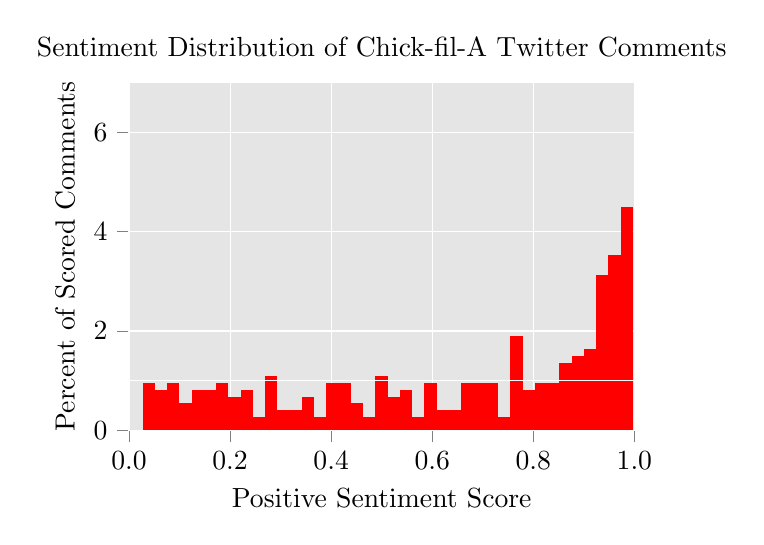
\begin{tikzpicture}

\begin{axis}[
axis background/.style={fill=white!89.80392156862746!black},
axis line style={white},
height=6cm,
tick align=outside,
tick pos=left,
title={Sentiment Distribution of Chick-fil-A Twitter Comments},
width=8cm,
x grid style={white},
xlabel={Positive Sentiment Score},
xmajorgrids,
xmin=0, xmax=1,
xtick={0,0.2,0.4,0.6,0.8,1},
xticklabels={0.0,0.2,0.4,0.6,0.8,1.0},
y grid style={white},
ylabel={Percent of Scored Comments},
ymajorgrids,
ymin=0, ymax=7
]
\draw[fill=red,draw opacity=0] (axis cs:0.0267013683915138,0) rectangle (axis cs:0.0509563982486725,0.952475100678047);
\draw[fill=red,draw opacity=0] (axis cs:0.0509564019739628,0) rectangle (axis cs:0.0752114355564117,0.816407166457287);
\draw[fill=red,draw opacity=0] (axis cs:0.0752114206552505,0) rectangle (axis cs:0.0994664505124092,0.952475027533502);
\draw[fill=red,draw opacity=0] (axis cs:0.0994664579629898,0) rectangle (axis cs:0.123721487820148,0.544271444304858);
\draw[fill=red,draw opacity=0] (axis cs:0.123721480369568,0) rectangle (axis cs:0.147976517677307,0.816407166457287);
\draw[fill=red,draw opacity=0] (axis cs:0.147976517677307,0) rectangle (axis cs:0.172231540083885,0.816407417238643);
\draw[fill=red,draw opacity=0] (axis cs:0.172231540083885,0) rectangle (axis cs:0.196486577391624,0.952474734955433);
\draw[fill=red,draw opacity=0] (axis cs:0.196486562490463,0) rectangle (axis cs:0.220741584897041,0.680339514365536);
\draw[fill=red,draw opacity=0] (axis cs:0.220741599798203,0) rectangle (axis cs:0.244996637105942,0.816406915676086);
\draw[fill=red,draw opacity=0] (axis cs:0.244996622204781,0) rectangle (axis cs:0.269251644611359,0.272135972933938);
\draw[fill=red,draw opacity=0] (axis cs:0.269251644611359,0) rectangle (axis cs:0.293506681919098,1.08854255423478);
\draw[fill=red,draw opacity=0] (axis cs:0.293506681919098,0) rectangle (axis cs:0.317761719226837,0.408203457838043);
\draw[fill=red,draw opacity=0] (axis cs:0.317761719226837,0) rectangle (axis cs:0.342016756534576,0.408203457838043);
\draw[fill=red,draw opacity=0] (axis cs:0.342016756534576,0) rectangle (axis cs:0.366271764039993,0.680339932334846);
\draw[fill=red,draw opacity=0] (axis cs:0.366271764039993,0) rectangle (axis cs:0.390526801347733,0.272135638558695);
\draw[fill=red,draw opacity=0] (axis cs:0.390526801347733,0) rectangle (axis cs:0.414781838655472,0.952474734955433);
\draw[fill=red,draw opacity=0] (axis cs:0.414781838655472,0) rectangle (axis cs:0.439036875963211,0.952474734955433);
\draw[fill=red,draw opacity=0] (axis cs:0.439036846160889,0) rectangle (axis cs:0.463291853666306,0.544271945867877);
\draw[fill=red,draw opacity=0] (axis cs:0.463291883468628,0) rectangle (axis cs:0.487546920776367,0.272135638558695);
\draw[fill=red,draw opacity=0] (axis cs:0.487546920776367,0) rectangle (axis cs:0.511801958084106,1.08854255423478);
\draw[fill=red,draw opacity=0] (axis cs:0.511801958084106,0) rectangle (axis cs:0.536056995391846,0.680339096396738);
\draw[fill=red,draw opacity=0] (axis cs:0.536056995391846,0) rectangle (axis cs:0.560312032699585,0.816406915676086);
\draw[fill=red,draw opacity=0] (axis cs:0.560312032699585,0) rectangle (axis cs:0.584567010402679,0.272136307310003);
\draw[fill=red,draw opacity=0] (axis cs:0.584567010402679,0) rectangle (axis cs:0.608822047710419,0.952474734955433);
\draw[fill=red,draw opacity=0] (axis cs:0.608822047710419,0) rectangle (axis cs:0.633077085018158,0.408203457838043);
\draw[fill=red,draw opacity=0] (axis cs:0.633077085018158,0) rectangle (axis cs:0.657332122325897,0.408203457838043);
\draw[fill=red,draw opacity=0] (axis cs:0.657332122325897,0) rectangle (axis cs:0.681587159633636,0.952474734955433);
\draw[fill=red,draw opacity=0] (axis cs:0.681587159633636,0) rectangle (axis cs:0.705842196941376,0.952474734955433);
\draw[fill=red,draw opacity=0] (axis cs:0.705842196941376,0) rectangle (axis cs:0.730097234249115,0.952474734955433);
\draw[fill=red,draw opacity=0] (axis cs:0.73009717464447,0) rectangle (axis cs:0.754352152347565,0.272136307310003);
\draw[fill=red,draw opacity=0] (axis cs:0.754352211952209,0) rectangle (axis cs:0.778607249259949,1.90494946991087);
\draw[fill=red,draw opacity=0] (axis cs:0.778607249259949,0) rectangle (axis cs:0.802862286567688,0.816406915676086);
\draw[fill=red,draw opacity=0] (axis cs:0.802862286567688,0) rectangle (axis cs:0.827117323875427,0.952474734955433);
\draw[fill=red,draw opacity=0] (axis cs:0.827117323875427,0) rectangle (axis cs:0.851372361183167,0.952474734955433);
\draw[fill=red,draw opacity=0] (axis cs:0.851372361183167,0) rectangle (axis cs:0.875627398490906,1.36067819279348);
\draw[fill=red,draw opacity=0] (axis cs:0.875627398490906,0) rectangle (axis cs:0.899882435798645,1.49674601207282);
\draw[fill=red,draw opacity=0] (axis cs:0.899882435798645,0) rectangle (axis cs:0.92413741350174,1.63281784386002);
\draw[fill=red,draw opacity=0] (axis cs:0.92413741350174,0) rectangle (axis cs:0.948392450809479,3.129559843425);
\draw[fill=red,draw opacity=0] (axis cs:0.948392450809479,0) rectangle (axis cs:0.972647488117218,3.53776330126304);
\draw[fill=red,draw opacity=0] (axis cs:0.972647488117218,0) rectangle (axis cs:0.996902525424957,4.49023803621847);
\path [draw=white, fill opacity=0] (axis cs:0,0)
--(axis cs:0,7);

\path [draw=white, fill opacity=0] (axis cs:1,0)
--(axis cs:1,7);

\path [draw=white, fill opacity=0] (axis cs:0,0)
--(axis cs:1,0);

\path [draw=white, fill opacity=0] (axis cs:0,1)
--(axis cs:1,1);

\end{axis}

\end{tikzpicture}